\documentclass[dvipsnames]{standalone}
\usepackage{tikz}

\usetikzlibrary{positioning}

\colorlet{line2line}{SkyBlue!50}

\newcommand{\stheight}{0.7cm}
\newcommand{\stshift}{0.3cm}

\begin{document}

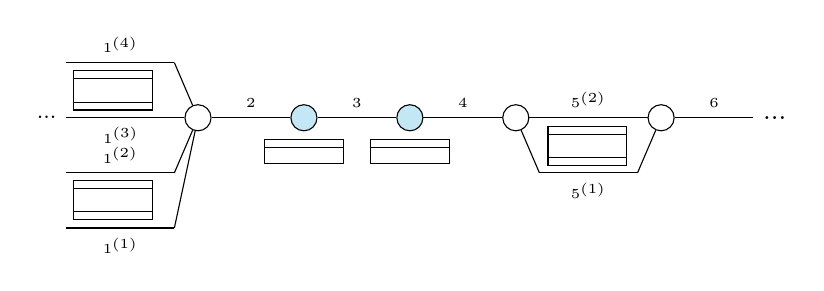
\begin{tikzpicture}[
    junction/.style={draw,circle},
    onesideplatform/.pic={
        \node[
            draw,rectangle,minimum height=0.3cm, minimum width=1cm
        ] (platform) {};
        \coordinate [above=0.05cm of platform.west] (x);
        \coordinate [above=0.05cm of platform.east] (y);
        \draw (x) -- (y);
    },
    twosideplatform/.pic={
        \node[
            draw,rectangle,minimum height=0.5cm, minimum width=1cm
        ] (platform) {};
        \coordinate [above=0.15cm of platform.west] (x);
        \coordinate [above=0.15cm of platform.east] (y);
        \coordinate [below=0.15cm of platform.west] (u);
        \coordinate [below=0.15cm of platform.east] (v);
        \draw (x) -- (y);
        \draw (u) -- (v);
    }
]

\node [] (start) {\footnotesize ...};
\node [junction, right=1.5cm of start] (A) {};
\node [junction, right=1cm of A, fill=line2line] (B) {};
\node [junction, right=1cm of B, fill=line2line] (C) {};
\node [junction, right=1cm of C] (D) {};
\node [junction, right=1.5cm of D] (E) {};
\node [right=1cm of E] (stop) {...};



\draw (start) -- (A) node[midway,below left=0.0cm and -0.29cm]{\tiny $1^{(3)}$};
\draw (A) -- (B) node[midway,above]{\tiny $2$};
\draw (B) -- (C) node[midway,above]{\tiny $3$};
\draw (C) -- (D) node[midway,above]{\tiny $4$};
\draw (D) -- (E) node[midway,above]{\tiny $5^{(2)}$};
\draw (E) -- (stop) node[midway,above]{\tiny $6$};

\coordinate [below right=\stheight and 0.25cm of start.center] (start1);
\coordinate [below left=\stheight and \stshift of A.center] (A1);
\draw (start1) -- (A1) node[midway, above]{\tiny $1^{(2)}$};
\draw (A1) -- (A);

\coordinate [above right=\stheight and 0.25cm of start.center] (start2);
\coordinate [above left=\stheight and \stshift of A.center] (A2);
\draw (start2) -- (A2) node[midway, above]{\tiny $1^{(4)}$};
\draw (A2) -- (A);

\coordinate [below right=2*\stheight and 0.25cm of start.center] (start3);
\coordinate [below left=2*\stheight and \stshift of A.center] (A3);
\draw (start3) -- (A3) node[midway, below]{\tiny $1^{(1)}$};
\draw (A3) -- (A);

\coordinate [below right=\stheight and \stshift of D.center] (D1);
\coordinate [below left=\stheight and \stshift of E.center] (E1);
\draw (D) -- (D1);
\draw (D1) -- (E1) node[midway,below]{\tiny $5^{(1)}$};
\draw (E1) -- (E);


\pic [below=0.1cm of B] {onesideplatform};
\pic [below=0.1cm of C] {onesideplatform};

\pic [below left=0.665cm and 0.45cm of A] {twosideplatform};
\pic [above left=-0.03cm and 0.45cm of A] {twosideplatform};

\pic [below right=-0.02cm and 0.28cm of D] {twosideplatform};
\end{tikzpicture}


\end{document}
